\section{Organizzazione del lavoro}

\subsection{Organizzazione del processo di sviluppo}
Per l’implementazione dei microservizi che compongono il sistema ServeEasy, attualmente delineato al primo zoom-in, è stato applicato un approccio “polyrepo"\cite{polyrepo}, definendo per ogni microservizio un’area di progetto dedicata. 

Scelta GitHub come piattaforma di hosting per il progetto software, un membro del team è stato incaricato del setup, controllo e gestione delle repository per i singoli microservizi.

Per raggiungere tale organizzazione, è stata prima di tutto creata un’area di lavoro per familiarizzare con le tecnologie selezionate, impiegando uno sforzo congiunto nello studio e prototipazione.

Nel processo di sviluppo sono state specificate delle regole mutualmente pattuite:
\begin{itemize}
    \item Nessuno esegue push diretto dall’area di lavoro locale verso il main branch: ognuno lavora esclusivamente sulla propria branch;
    \item Nei commit e nelle pull requests va espressa una sintesi del proprio lavoro svolto;
\item Cambiamenti importanti vanno discussi;
\item Ogni implementazione va testata;
\item Prima di effettuare una merge sul main branch, l’implementazione deve aver passato le fasi di build e di test con successo.
\end{itemize}

A supporto del processo di sviluppo, sono state introdotte automatizzazioni per garantire Continuous Integration e Continuous Delivery, servendosi di Github Workflows e Docker allo scopo di aumentare la velocità di deployment delle nuove modifiche apportate, garantendo al contempo integrità:
\begin{itemize}
    \item Un evento di push verso il proprio branch causa l’avvio della job di CI posta a sorveglianza del proprio spazio di lavoro sulla repository, allo scopo di effettuare un controllo di compilazione;
    \item Un evento verso il main branch (quale, ad esempio, una merge) causa l’avvio della job di CI/CD posta a sorveglianza del main sulla repository, la quale effettua un controllo di compilazione, genera un eseguibile e procede con le fasi di build e ship dell'immagine Docker corrispondente verso il registry DockerHub \cite{DockerOverview}.
\end{itemize}

In particolare, nel punto 2 si parla di Continuous Delivery e non Continuous Deployment, in quanto il deployment della nuova immagine va eseguita manualmente \cite{CDDocker}.

Il deployment verrà effettuato tramite Docker Compose: vengono definiti in un unico file i servizi offerti dal registry di riferimento (Dockerhub), le loro caratteristiche e dipendenze, cosicchè sarà sufficiente avviare il file per poter scaricare le immagini dei microservizi e servizi d’interesse in una rete di container dedicata.



\begin{figure}[htbp]
	\centering
	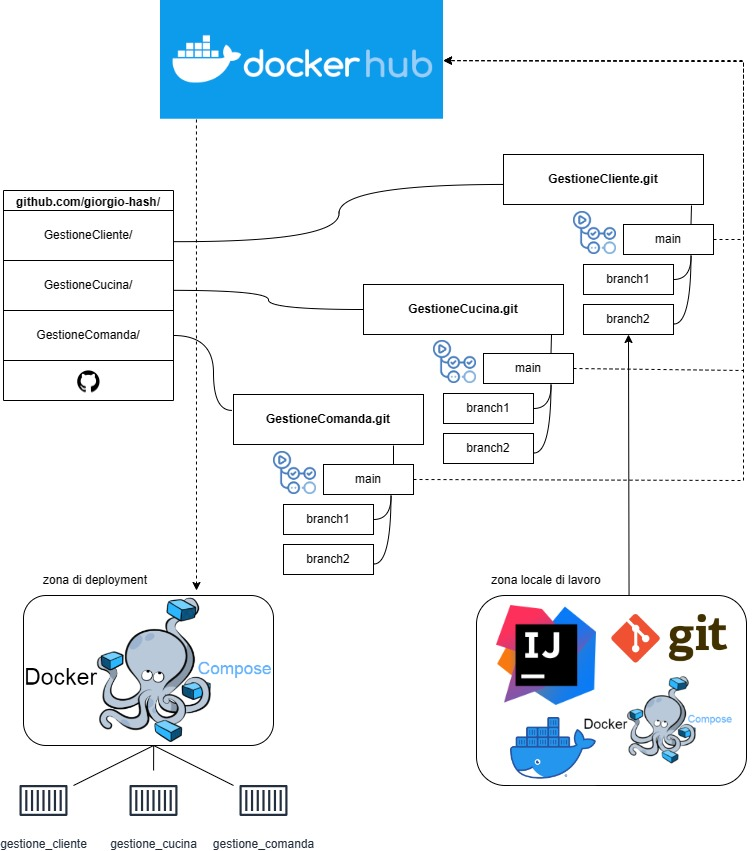
\includegraphics[scale=0.36]{iterazione1/images/DevOps.jpg}
	\caption{Organizzazione del lavoro cloud e locale, CI/CD e deployment 
 \label{fig:devopsit1}}
\end{figure}


\subsection{Organizzazione dell'area di lavoro}
Oltre all'IDE di Intellij IDEA e Git, l'area di lavoro locale è supportata da Docker Compose per attivare i servizi a supporto dell'esecuzione del singolo microservizio: non solo dipendenze, quali Kafka, Zookeeper ed il database MariaDB, ma anche strumenti utili per la visualizzazione ed interazione ad alto livello col sistema, quali:
\begin{itemize}
    \item Kafdrop per monitorare i messaggi passati tra pub e sub attraverso Kafka;
    \item PHPMyAdmin per monitorare, sviluppare ed iniettare dati nel database MariaDB.
\end{itemize}
Facendo leva sulla portabilità offerta dal framework Docker, viene garantito un ambiente altamente personalizzabile, flessibile e di facile implementazione. 

\begin{figure}[htbp]
	\centering
	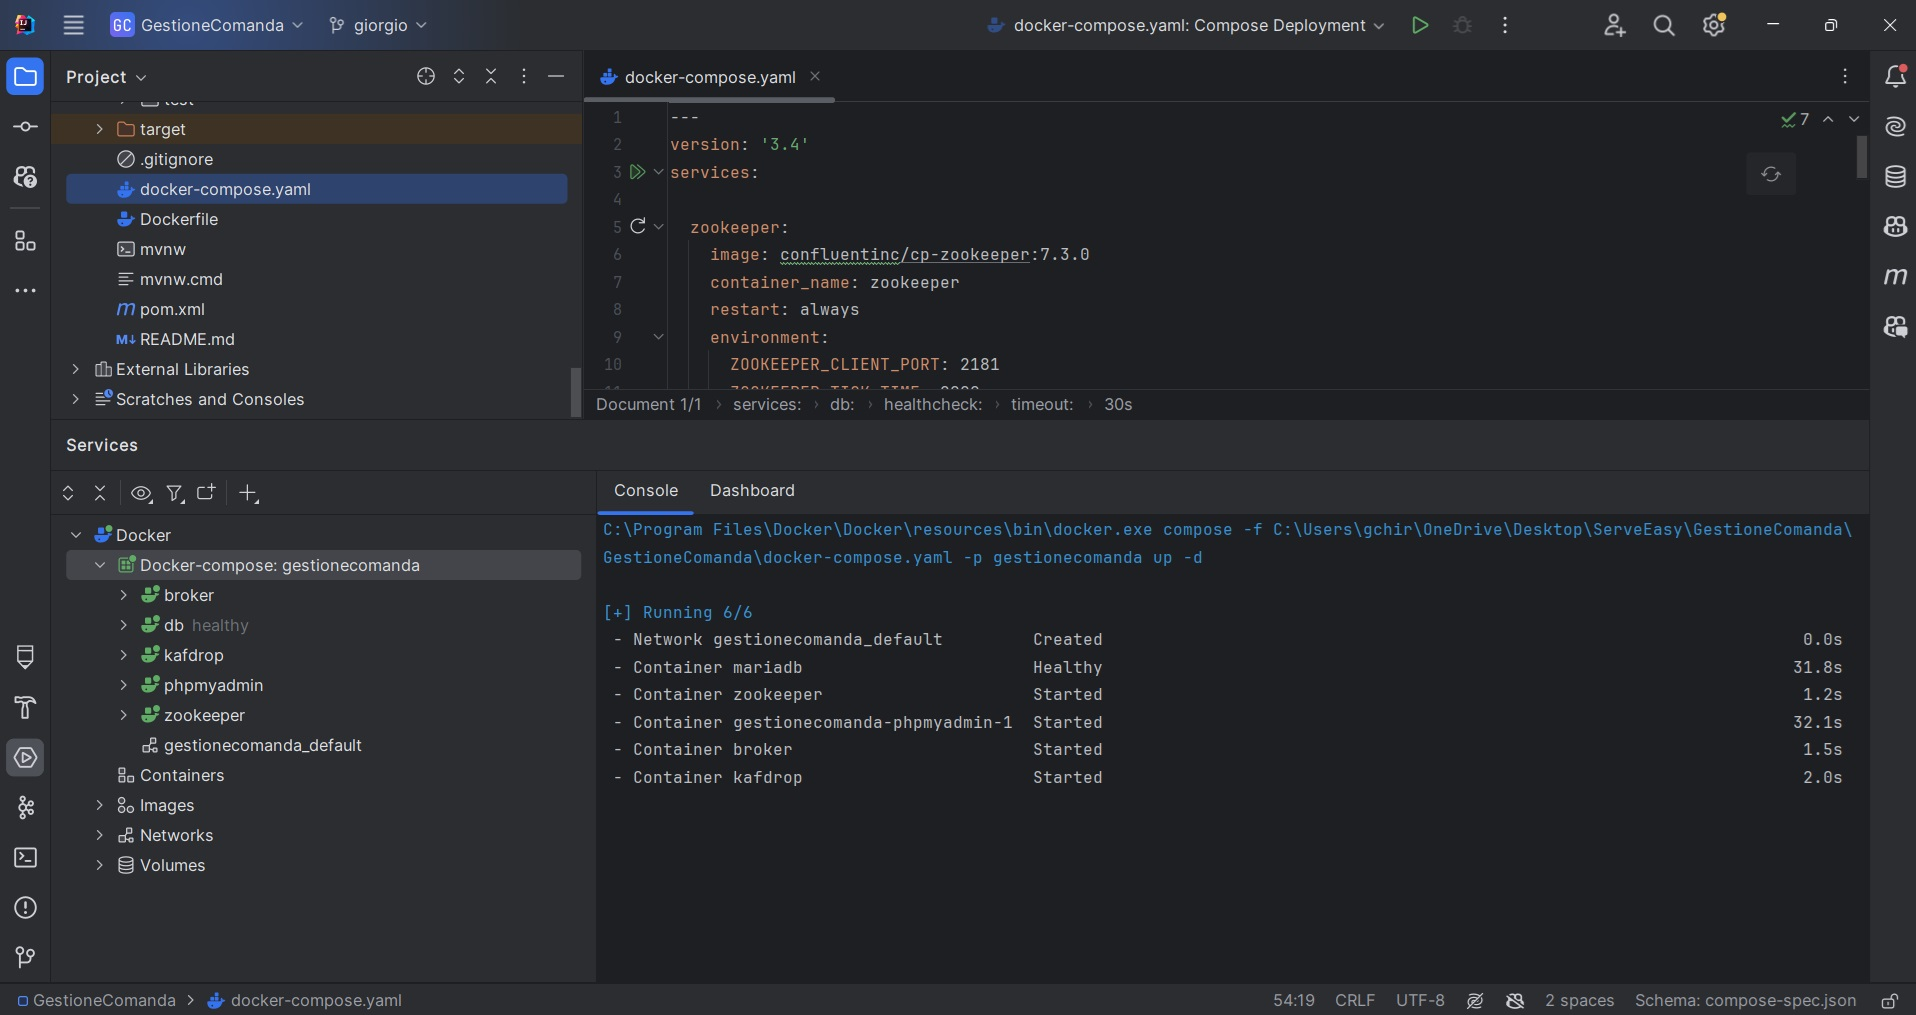
\includegraphics[scale=0.36]{iterazione1/images/IDEIDEA.jpg}
	\caption{Ambiente di lavoro con Intellij IDEA e Docker Compose
 \label{fig:IDEAit1}}
\end{figure}

\begin{figure}[htbp]
	\centering
	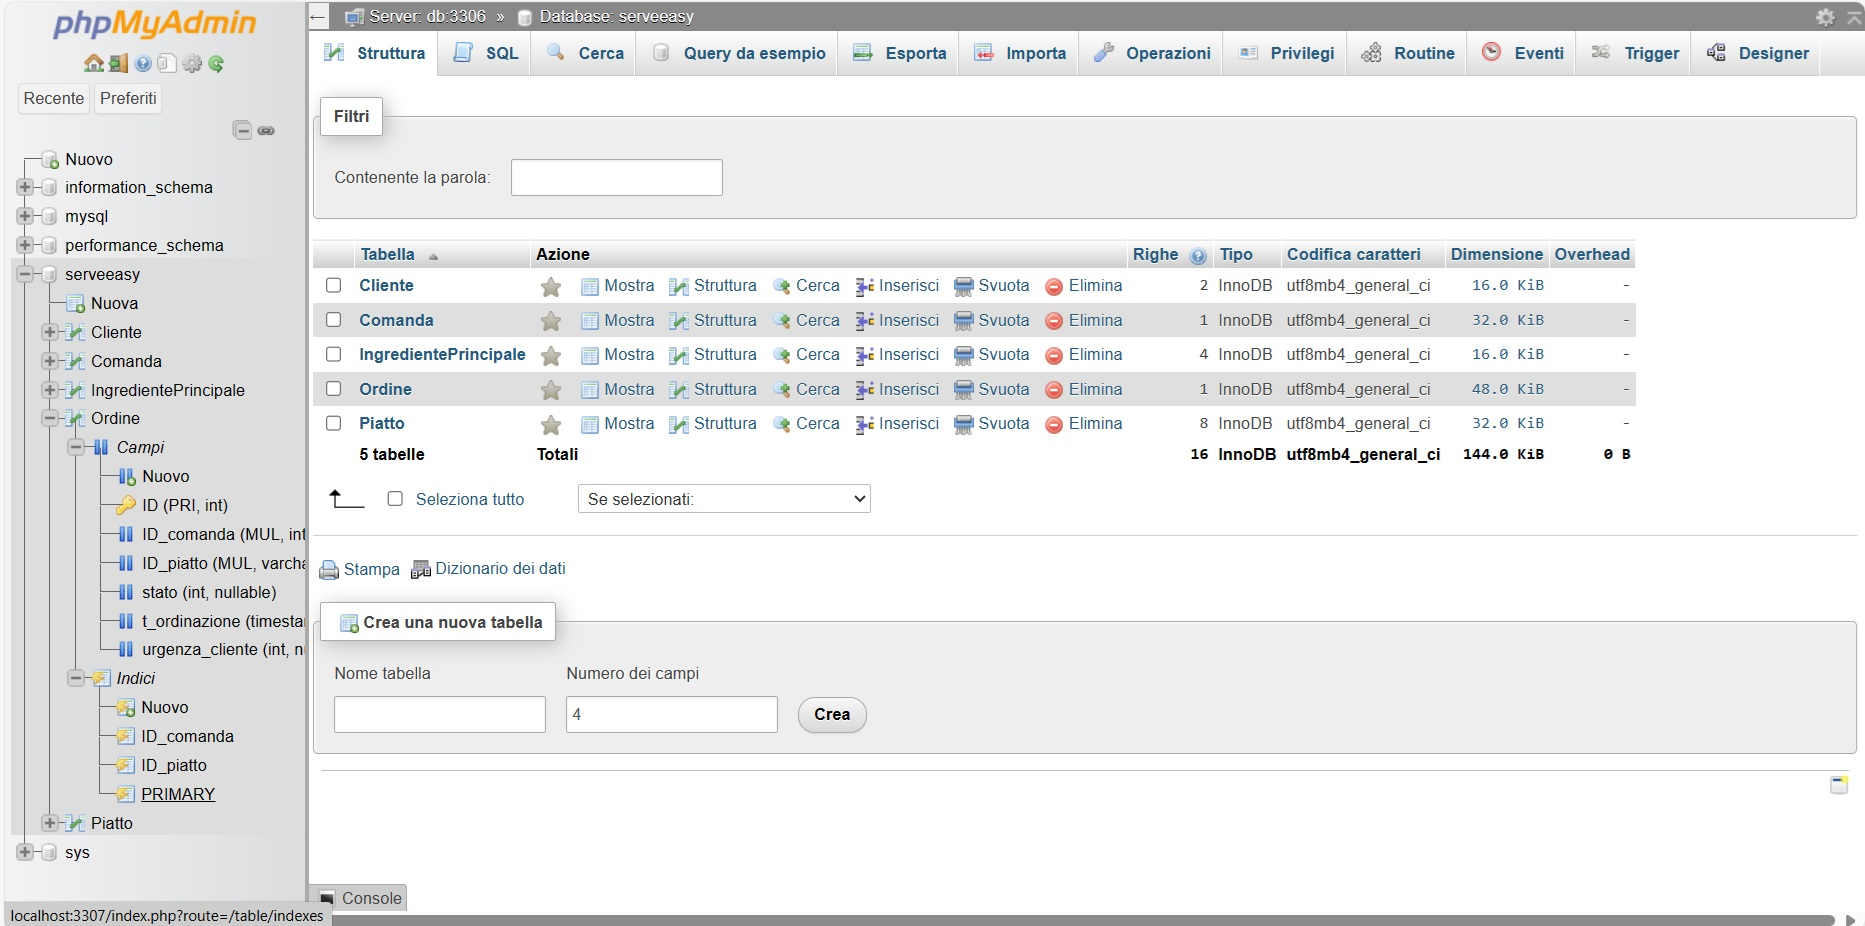
\includegraphics[scale=0.36]{iterazione1/images/phpmyadmin.jpg}
	\caption{interfaccia grafica di PHPMyAdmin eseguito da container
 \label{fig:phpmyadmin}}
\end{figure}

Fin dal principio, l'area di lavoro è dotata della source tree che esplicita il layout dei subsystem identificati in fase di progettazione (paragrafo 2.3), comprendendo inoltre la cartella interfunzionale \textit{config}, necessaria per contenere gli artefatti di configurazione delle funzionalità (ad es. per JPA).

Alla radice del progetto, vi è inoltre una cartella dedicata a contenere dati di persistenza (cartella \textit{/db}).

\begin{figure}[htbp]
	\centering
	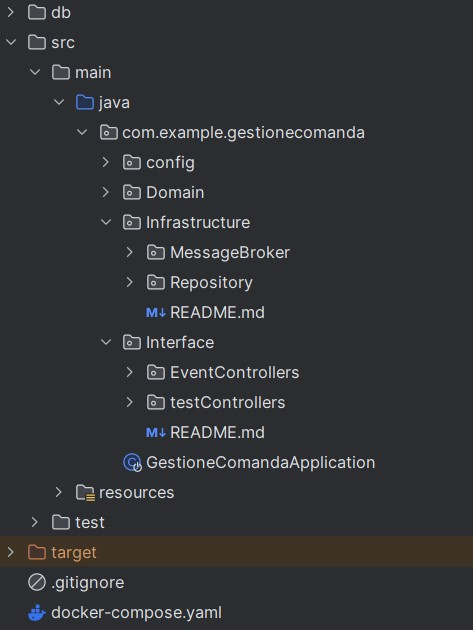
\includegraphics[scale=0.50]{iterazione1/images/source tree.jpg}
	\caption{source tree del progetto GestioneComanda
 \label{fig:srctreeGestioneComanda}}
\end{figure}

L'applicativo viene costruito per essere eseguito su \textit{localhost:8080}. Lo sviluppo in locale è impostato per risolvere le dipendenze di rete tramite il framework Docker: i servizi offerti da database e message broker vengono quindi sempre esposti su porte distinte dell'interfaccia di rete \textit{localhost}.
\clearpage